
\documentclass[a4paper,12pt]{report}

    \usepackage[english]{babel}
    \usepackage{graphicx}
    \linespread{1.5}
    \title{Implementation and Evaluation of Routing Algorithm in GENI Software-Defined Networking}
    \author{Wei-Hen Hsu}
    \date{\today}
    \begin{document}
    \maketitle{}
    \tableofcontents{}
    \begin{figure}
      \caption{A picture of a gull.}
      \centering
        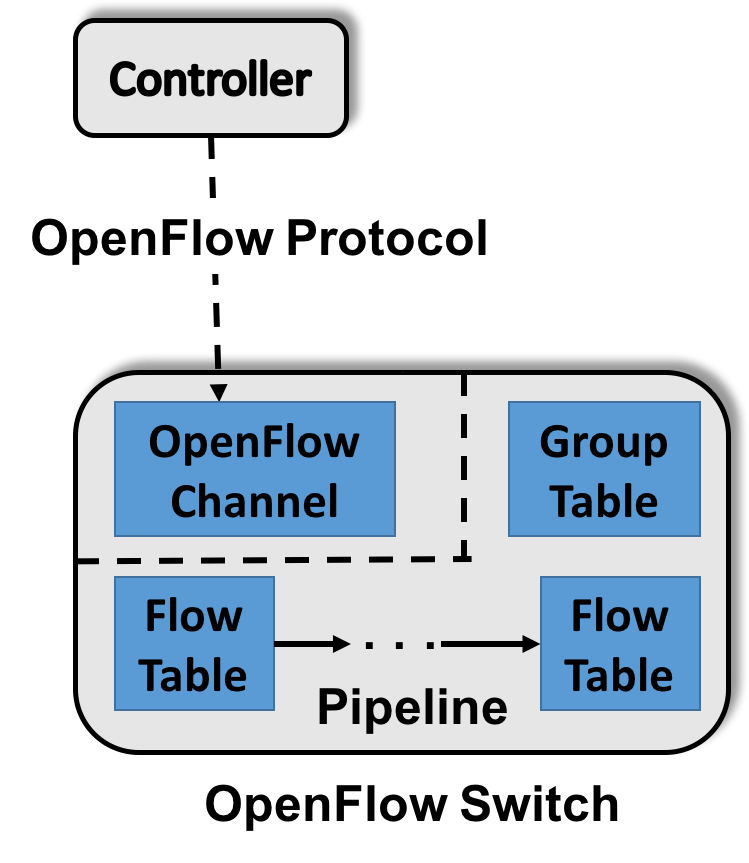
\includegraphics[width=0.5\textwidth]{OpenFlow.png}
    \end{figure}
    
    \begin{figure}
      \centering
        \reflectbox{%
          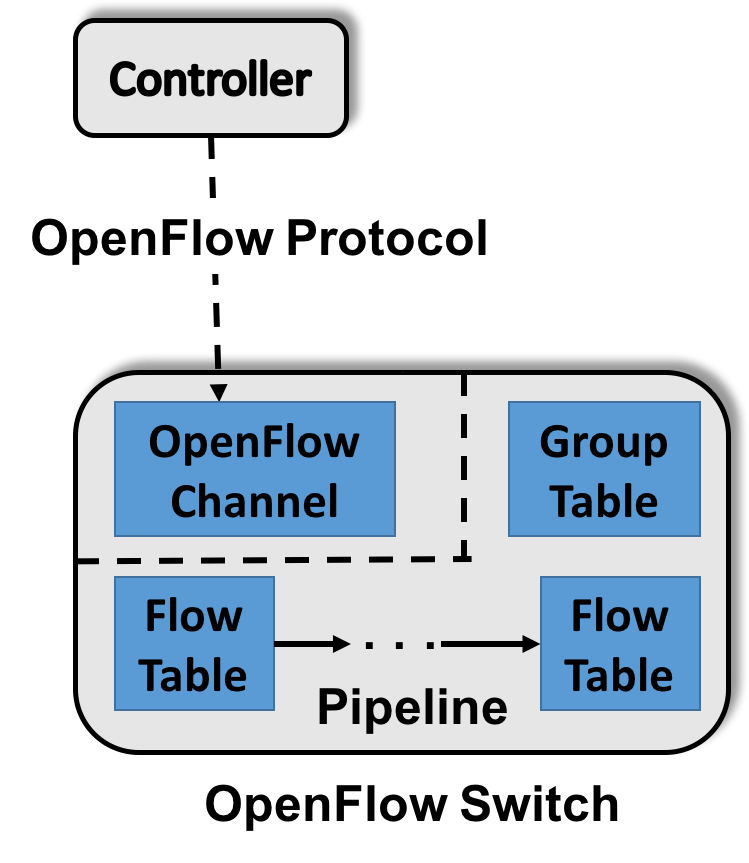
\includegraphics[width=0.5\textwidth]{OpenFlow.png}}
      \caption{A picture of the same gull
               looking the other way!}
    \end{figure}
    
    \begin{table}
      \centering
        \begin{tabular}{| l c r |}
        \hline
        1 & 2 & 3 \\
        4 & 5 & 6 \\
        7 & 8 & 9 \\
        \hline
        \end{tabular}
      \caption{A simple table}
    \end{table}
    
    Notice how the tables and figures
    have independent counters.
    
    \end{document}